%%
%% Autonomous AI Paper -- engrXiv Preprint Format
%% Paper #3 in the AI Systems Landscape 2026 series
%% License: CC BY 4.0
%%
\documentclass[12pt, a4paper]{article}

%% ================================================================
%% PACKAGES
%% ================================================================
\usepackage[utf8]{inputenc}
\usepackage[T1]{fontenc}
\usepackage{lmodern}
\usepackage[margin=1in]{geometry}
\usepackage{setspace}
\onehalfspacing

\usepackage{booktabs}
\usepackage{multirow}
\usepackage{tikz}
\usetikzlibrary{shapes.geometric, arrows.meta, positioning, calc, fit, backgrounds, decorations.pathreplacing}
\usepackage{pgfplots}
\pgfplotsset{compat=1.18}
\usepackage{algorithm}
\usepackage{algpseudocode}
\usepackage{subcaption}
\usepackage{amsmath,amssymb,amsthm}
\usepackage{natbib}
\bibliographystyle{plainnat}
\usepackage{graphicx}
\usepackage{xcolor}
\usepackage[breaklinks=true,colorlinks=true,linkcolor=blue!70!black,citecolor=green!50!black,urlcolor=blue!70!black]{hyperref}
\usepackage{url}
% orcidlink removed and replaced with a plain hyperlink for preprint compatibility

%% ================================================================
%% THEOREM ENVIRONMENTS
%% ================================================================
\newtheorem{definition}{Definition}
\newtheorem{proposition}{Proposition}

%% ================================================================
%% PREPRINT HEADER
%% ================================================================
\usepackage{fancyhdr}
\setlength{\headheight}{15pt}
\pagestyle{fancy}
\fancyhf{}
\renewcommand{\headrulewidth}{0.4pt}
\lhead{\small engrXiv Preprint | CC BY 4.0}
\rhead{\small\thepage}
\lfoot{\small AI Systems Landscape 2026, Paper \#3}
\rfoot{\small July 2026}

%% ================================================================
\begin{document}

%% ================================================================
%% TITLE PAGE
%% ================================================================
\begin{center}
    {\Large\bfseries Autonomy Without Agency:\\[4pt]
    A Formal Distinction Between Autonomous and Agentic AI Systems\\[2pt]
    in Safety-Critical Domains}

    \vspace{1em}

    {\large Hameem Mahdi}\\[2pt]
    {\small \href{https://orcid.org/0009-0007-0005-3080}{ORCID: 0009-0007-0005-3080}}\\[4pt]
    Mayo Clinic, Rochester, MN, USA\\
    \texttt{mahdi.hameem@mayo.edu}

    \vspace{1em}

    {\small\textbf{Preprint} (Not yet peer-reviewed)}\\[2pt]
    {\small Submitted to engrXiv, July 2026}\\[2pt]
    {\small engrXiv: Engineering Open Archive (engrxiv.org)}\\[2pt]
    {\small License: \href{https://creativecommons.org/licenses/by/4.0/}{CC BY 4.0 International}}\\[2pt]
    {\small Paper \#3 in the \emph{AI Systems Landscape 2026} series}
\end{center}

\vspace{1em}

%% ================================================================
%% ABSTRACT
%% ================================================================
\begin{abstract}
\noindent
The AI discourse conflates two fundamentally distinct paradigms, \emph{autonomous} and \emph{agentic} AI, under a shared vocabulary of ``AI that acts independently.'' This conflation obscures critical architectural differences that carry profound implications for safety, governance, and regulatory compliance, particularly in safety-critical domains such as aviation, industrial control, algorithmic trading, and clinical decision support. This paper provides the first formal, criterion-based distinction between Autonomous AI (Non-Agentic) and Agentic AI, grounded in six architectural dimensions: goal origin, tool selection, reasoning mechanism, self-correction capacity, memory architecture, and operational scope. We formalise the \textsc{Autonomy Loop} as a five-phase closed-loop cycle (Monitor, Decide, Act, Verify, and Loop) and contrast it against the open-ended PPAS (Perceive-Plan-Act-Self-Correct) agent loop from classical agent theory. We systematically map 19 production systems across four sub-types (Continuous Control, Event-Driven, Scheduled/Pipeline, and Autonomous Decision Systems) mapped to an 8-layer technology stack spanning sensor data through governance and oversight. Our empirical survey demonstrates that autonomous systems operating within pre-defined operational envelopes dominate high-assurance domains: algorithmic trading accounts for 60 to 75\% of US equity volume, Kubernetes-based auto-scaling underpins approximately 85\% of cloud production workloads, and civil aviation autopilots manage 95\% of flight time. We quantify seven fundamental limitations of non-agentic autonomy and map the resulting risk taxonomy against the EU AI Act, GDPR Article 22, MiFID~II, FAA/EASA regulations, and FDA Software as a Medical Device (SaMD) frameworks. The formal distinction introduced here provides system designers, regulators, and safety engineers with precise vocabulary to govern the deployment of autonomous systems in high-stakes contexts, and clarifies the boundary conditions under which upgrading a system from autonomous to agentic operation introduces qualitatively new risks. All data and analysis artefacts are publicly available as part of the AI Systems Landscape 2026 repository.
\end{abstract}

\medskip

\noindent\textbf{Keywords:} Autonomous AI, Agentic AI, Closed-Loop Control, Safety-Critical Systems, Operational Envelope, AIOps, Algorithmic Trading, AI Governance, EU AI Act, GDPR Article 22, Autonomy Loop

\newpage

%% ================================================================
%% SECTION 1: INTRODUCTION
%% ================================================================
\section{Introduction}\label{sec:intro}

\subsection{Background and Motivation}
As artificial intelligence increasingly performs consequential actions without direct human authorisation (scaling cloud infrastructure, executing financial trades, moderating social media content, and controlling physical processes), the vocabulary used to describe these systems matters enormously. Terms such as ``autonomous,'' ``agentic,'' ``self-directed,'' and ``intelligent'' are deployed interchangeably in industry discourse, regulatory filings, and academic literature, creating ambiguity about what level of autonomy a given system actually possesses, what risks it presents, and which regulatory frameworks apply.

This conflation is not merely academic. When regulators ask whether a system is ``autonomous,'' they are asking whether it requires human-in-the-loop approval for each decision, a question with direct legal consequences under GDPR Article 22~\citep{eu2016gdpr}, the EU AI Act~\citep{eu2024aiact}, MiFID~II algorithmic trading provisions~\citep{mifid2014}, and FDA Software as a Medical Device guidance~\citep{fda2019samd}. When safety engineers ask the same question, they are asking about failure mode characteristics, blast radius, and recovery time, all of which differ fundamentally between autonomous and agentic architectures.

\subsection{The Core Conflation}
The AI field currently uses ``autonomous'' to describe at least two architecturally distinct paradigms:

\begin{description}
    \item[Autonomous (Non-Agentic) AI] Systems that execute pre-defined policies within constrained operational envelopes, without human approval for individual decisions, but operating within boundaries set entirely by humans at design time. Examples include aircraft autopilots, Kubernetes Horizontal Pod Autoscalers, high-frequency trading engines, and SCADA-controlled industrial processes.
    \item[Agentic AI] Systems that receive high-level goals, decompose them into sub-tasks, dynamically select and invoke tools, maintain persistent memory across reasoning steps, and self-correct from failures, all within operator-defined guardrails but without pre-scripted decision policies. Examples include LLM-based coding agents~\citep{mahdi2026agentic}, research agents, and multi-agent enterprise workflows.
\end{description}

These two paradigms differ not in degree of autonomy but in kind: autonomous systems execute policy; agentic systems reason about which policy to follow. This distinction has profound implications for verification, testing, safety analysis, and regulation.

\subsection{Research Objectives}
This paper addresses the conflation through five research questions:

\begin{description}
    \item[RQ1] What formal criteria distinguish Autonomous (Non-Agentic) AI from Agentic AI along architectural dimensions?
    \item[RQ2] How does the 5-phase Autonomy Loop differ from classical agent loop models, and what are the implications for safety analysis?
    \item[RQ3] What are the dominant sub-types of Autonomous AI in production, and how do they map to a common 8-layer technology stack?
    \item[RQ4] What fundamental limitations does the non-agentic autonomy model impose, and how do these limitations create safety guarantees absent in agentic systems?
    \item[RQ5] How do existing regulatory frameworks map to autonomous versus agentic systems, and where do governance gaps exist?
\end{description}

\subsection{Contributions}
Our main contributions are:
\begin{enumerate}
    \item A formal six-dimension criterion set for distinguishing Autonomous AI from Agentic AI, with operational tests for each criterion.
    \item Formalisation of the \textsc{Autonomy Loop} as a five-phase closed-loop control cycle and its comparison against PPAS and classical agent models.
    \item A comprehensive taxonomy of four Autonomous AI sub-types mapped to an 8-layer technology stack with 30+ platform examples.
    \item An empirical characterisation of production autonomous systems across six industries, including quantitative adoption metrics.
    \item A seven-point risk taxonomy for autonomous systems with mitigations and a regulatory mapping across five major frameworks.
    \item A boundary condition analysis identifying the precise conditions under which autonomous-to-agentic upgrades introduce qualitatively new safety risks.
\end{enumerate}

\subsection{Paper Organisation}
Section~\ref{sec:background} reviews related work and classical control theory. Section~\ref{sec:distinction} formalises the autonomous/agentic distinction. Section~\ref{sec:loop} presents the Autonomy Loop. Section~\ref{sec:stack} maps the 8-layer stack. Section~\ref{sec:subtypes} analyses sub-types. Section~\ref{sec:platforms} surveys platforms and tools. Section~\ref{sec:usecases} presents industry use cases. Section~\ref{sec:evaluation} covers benchmarks and metrics. Section~\ref{sec:market} provides market analysis. Section~\ref{sec:risks} analyses risks. Section~\ref{sec:governance} covers regulation. Section~\ref{sec:future} identifies open problems. Section~\ref{sec:conclusion} concludes.

%% ================================================================
%% SECTION 2: BACKGROUND & RELATED WORK
%% ================================================================
\section{Background \& Related Work}\label{sec:background}

\subsection{Classical Control Theory and Autonomy}
The intellectual foundations of Autonomous AI predate digital computing. Wiener's cybernetics~\citep{wiener1948cybernetics} established the closed-loop feedback paradigm: a system that measures output, compares it to a reference, and adjusts input to minimise error. This principle underlies every autonomous system discussed in this paper, from aircraft autopilots (which maintain altitude by adjusting control surfaces based on barometric sensor feedback) to cloud auto-scalers (which adjust instance counts based on CPU utilisation metrics).

PID (Proportional-Integral-Derivative) controllers~\citep{astrom2006pid} operationalised closed-loop control in industrial processes, becoming the dominant technology in the Distributed Control Systems (DCS) that manage chemical plants, power stations, and manufacturing lines. The critical property of PID control, and of all classical autonomous systems, is \emph{predictability}: given the same input state, the system produces the same output action, and the action space is finite and fully specified at design time.

\subsection{Autonomy in Computing Systems}
IBM's Autonomic Computing manifesto~\citep{kephart2003autonomic} introduced four self-* properties: self-configuring, self-healing, self-optimising, and self-protecting, as the target for enterprise IT systems. This vision directly anticipates modern cloud auto-scaling and AIOps platforms, which implement all four properties within pre-defined operational envelopes. The autonomic computing framework explicitly distinguishes between the \emph{policy} that defines what the system should do and the \emph{autonomic elements} that execute that policy, a distinction central to our formal criterion set.

\subsection{SAE Levels of Driving Automation}
The SAE International standard J3016~\citep{sae2021j3016} provides the most widely deployed taxonomy of autonomous system capability, defining six levels of driving automation (0 to 5) based on who performs the dynamic driving task, who monitors the driving environment, and who is the fallback performer. SAE levels 0 to 2 involve human performance of the driving task (with varying levels of driver assistance); levels 3 to 5 involve Automated Driving System (ADS) performance. Crucially, even SAE Level 5 (full driving automation in all conditions) does not make a vehicle \emph{agentic}: the system still executes a pre-defined policy (drive safely to the destination) rather than reasoning about what goal to pursue or dynamically selecting which tools to use.

\subsection{Agent Theory}
Russell and Norvig~\citep{russell2021artificial} define an agent as ``anything that can be viewed as perceiving its environment through sensors and acting upon that environment through actuators.'' Under this broad definition, an aircraft autopilot and a GPT-4o-based coding agent are both agents. The distinction lies in the policy type: the autopilot follows a closed-form control law; the LLM agent synthesises plans using general-purpose reasoning. The BDI (Belief-Desire-Intention) model~\citep{rao1995bdi} captures the more restricted notion of a \emph{goal-directed} agent that maintains explicit beliefs about the world, desires representing goals, and intentions representing committed plans. Our formal criterion set operationalises this distinction into testable properties.

\subsection{Related Surveys}
Wang et al.~\citep{wang2024survey} survey LLM-based autonomous agents but use ``autonomous'' to mean both agentic and non-agentic systems. Duan et al.~\citep{duan2022survey} survey autonomous systems in physical domains without distinguishing the agentic dimension. To our knowledge, no prior work provides a formal, multi-criterion boundary between autonomous and agentic AI applicable across domains. The companion paper in this series~\citep{mahdi2026taxonomy} introduces a unified 19-type taxonomy; the present paper deepens the autonomous/agentic boundary within that taxonomy.

%% ================================================================
%% SECTION 3: FORMAL DISTINCTION
%% ================================================================
\section{Formal Distinction: Autonomous vs.\ Agentic AI}\label{sec:distinction}

\subsection{The Six Architectural Dimensions}

We propose six dimensions along which Autonomous (Non-Agentic) AI and Agentic AI differ fundamentally. For each dimension we provide a formal criterion and an operational test.

\begin{table}[ht]
\centering
\caption{Six-dimension formal distinction between Autonomous (Non-Agentic) AI and Agentic AI.}
\label{tab:distinction}
\begin{tabular}{p{3cm}p{5cm}p{5cm}}
\toprule
\textbf{Dimension} & \textbf{Autonomous (Non-Agentic)} & \textbf{Agentic} \\
\midrule
\textbf{Goal Origin}
  & Pre-defined at design time by humans. The system executes a fixed objective; it cannot modify its own goal.
  & Self-decomposed from a high-level human objective. The system formulates sub-goals at runtime. \\
\addlinespace
\textbf{Tool Selection}
  & Fixed. The system uses a specific, pre-configured set of actions (APIs, actuators, control outputs) defined at design time.
  & Dynamic. The system selects tools from an available set based on reasoning about the current task. \\
\addlinespace
\textbf{Reasoning Mechanism}
  & Policy execution. Decisions follow a pre-specified mapping (rule, model, controller) from state to action. No open-ended reasoning.
  & Multi-step planning. The system synthesises novel plans by reasoning about goals, context, and available tools. \\
\addlinespace
\textbf{Self-Correction}
  & Pre-defined fallback behaviour. Recovery follows scripted contingency logic specified at design time.
  & Dynamic re-planning. The system diagnoses failure and generates a new plan; recovery is not pre-scripted. \\
\addlinespace
\textbf{Memory Architecture}
  & Task-scoped state. Persistent state is limited to the variables required for the current operational loop; no episodic memory across tasks.
  & Persistent episodic memory. The system accumulates experience across tasks and uses it to inform future reasoning. \\
\addlinespace
\textbf{Operational Scope}
  & Narrow and formally bounded. The operational envelope is explicitly specified; out-of-envelope conditions trigger escalation or safe-fail.
  & Open-ended within guardrails. The system can pursue novel approaches to achieve its goal within operator-defined constraints. \\
\bottomrule
\end{tabular}
\end{table}

\subsection{Operational Tests}

The following operational tests allow practitioners to classify a system along each dimension:

\begin{enumerate}
    \item \textbf{Goal Origin Test:} Can the system modify its own objective without human intervention? \emph{Yes}: potentially agentic; \emph{No}: autonomous.
    \item \textbf{Tool Selection Test:} At runtime, does the system choose which tools/actions to invoke, or execute a pre-specified action sequence? \emph{Dynamic selection}: agentic; \emph{pre-specified}: autonomous.
    \item \textbf{Reasoning Test:} Can the system solve a problem type it was not explicitly programmed for? \emph{Yes}: agentic; \emph{No}: autonomous.
    \item \textbf{Self-Correction Test:} Does the system generate novel recovery strategies at runtime, or follow a pre-scripted fallback? \emph{Novel recovery}: agentic; \emph{scripted}: autonomous.
    \item \textbf{Memory Test:} Does the system's behaviour change based on experience from previous, distinct tasks? \emph{Yes}: agentic; \emph{No}: autonomous.
    \item \textbf{Scope Test:} Is the system's operational envelope formally specified and finite? \emph{Yes, finite}: autonomous; \emph{open-ended}: agentic.
\end{enumerate}

\begin{proposition}[Formal Criterion]
A system $S$ is classified as \emph{Autonomous (Non-Agentic)} if and only if it satisfies all six autonomous criteria simultaneously: pre-defined goals, fixed tool selection, policy-based reasoning, scripted self-correction, task-scoped memory, and formally bounded operational scope.
\end{proposition}

Note that real-world systems may occupy intermediate positions. A cloud auto-scaler is purely autonomous; an LLM-powered DevOps agent is purely agentic; a reinforcement-learning trading system that learns new strategies from market experience occupies an intermediate position. Our classification is not binary in practice but provides clear poles for anchoring analysis.

\subsection{Safety Implications of the Distinction}

The autonomous/agentic distinction carries direct safety implications:

\begin{itemize}
    \item \textbf{Formal verifiability.} Autonomous systems with finite, pre-specified action spaces are amenable to formal verification methods (model checking, Lyapunov stability analysis, safety envelopes). Agentic systems with open-ended reasoning are not, in general, formally verifiable.
    \item \textbf{Failure mode predictability.} In autonomous systems, failure modes can be enumerated at design time and tested exhaustively. In agentic systems, failure modes include unbounded plan generation and emergent tool-use patterns that cannot be fully anticipated.
    \item \textbf{Blast radius control.} Autonomous systems operate within a formally bounded authority envelope; blast radius is bounded by design. Agentic systems require guardrails to constrain blast radius, and those guardrails may be circumvented by novel reasoning strategies.
    \item \textbf{Regulatory compliance.} Autonomous systems in regulated domains can demonstrate compliance through conformance testing against specifications. Agentic systems require runtime monitoring and probabilistic compliance assurance, which existing regulatory frameworks do not yet fully accommodate.
\end{itemize}

%% ================================================================
%% SECTION 4: THE AUTONOMY LOOP
%% ================================================================
\section{The Autonomy Loop}\label{sec:loop}

\subsection{Formal Definition}

We formalise the Autonomous AI operational cycle as the \textsc{Autonomy Loop}: a five-phase closed-loop process that enables continuous, unsupervised operation within a pre-defined operational envelope.

\begin{definition}[Autonomous System]
An autonomous system $\mathcal{A} = \langle \mathcal{S}, \pi, \mathcal{E}, \mathcal{B}, \mathcal{L} \rangle$ is a tuple where $\mathcal{S}$ is a state space representing the observable environment, $\pi: \mathcal{S} \rightarrow \mathcal{A}ct$ is a pre-specified decision policy, $\mathcal{E}$ is an operational envelope (a bounded subset of $\mathcal{S}$), $\mathcal{B}$ is a fallback behaviour triggered when $s \notin \mathcal{E}$, and $\mathcal{L}$ is an immutable audit log.
\end{definition}

\begin{definition}[Autonomy Loop]
Given a system $\mathcal{A}$ and an environment state $s_t \in \mathcal{S}$, the Autonomy Loop executes iteratively:
\begin{enumerate}
    \item \textsc{Monitor}: $s_t = \text{observe}(\mathcal{S}, t)$: continuously collect telemetry, sensor readings, event streams, and derived metrics.
    \item \textsc{Decide}: $a_t = \pi(s_t)$: apply the decision policy to determine the appropriate action; if $s_t \notin \mathcal{E}$, invoke $\mathcal{B}$ (escalate or safe-fail).
    \item \textsc{Act}: execute $a_t$ within the authority boundary (no human approval required).
    \item \textsc{Verify}: $v_t = \text{verify}(s_{t+1}, a_t)$: confirm the action achieved its intended effect; detect anomalous outcomes.
    \item \textsc{Loop}: $\log(\mathcal{L}, s_t, a_t, v_t)$; return to Step 1.
\end{enumerate}
The loop repeats indefinitely; humans set boundaries ($\mathcal{E}$, $\mathcal{B}$, $\pi$) but do not participate in individual iterations.
\end{definition}

\subsection{Comparison with Classical Agent Loop Models}

\begin{table}[ht]
\centering
\caption{Comparison of control and agent loop models.}
\label{tab:loop-comparison}
\begin{tabular}{lcccccc}
\toprule
\textbf{Model} & \textbf{Phases} & \textbf{Memory} & \textbf{Open Policy} & \textbf{Self-Correct} & \textbf{Domain} \\
\midrule
PID Controller~\citep{astrom2006pid}         & 1 & None      & No  & Via feedback & Industrial control \\
Autonomic Computing~\citep{kephart2003autonomic} & 4 & System state & No & Via self-* rules & IT operations \\
OODA Loop~\citep{boyd1987ooda}               & 4 & Implicit  & Limited & Limited & Military/tactical \\
BDI Agent~\citep{rao1995bdi}                 & 3 & Explicit  & Yes & Via re-planning & Symbolic agents \\
\textbf{Autonomy Loop (Ours)}                & 5 & Task-scoped & No & Via $\mathcal{B}$ (scripted) & Safety-critical \\
PPAS (Agentic)~\citep{mahdi2026agentic}      & 4 & Episodic  & Yes & Dynamic & LLM agents \\
\bottomrule
\end{tabular}
\end{table}

\subsection{TikZ Diagram}

\begin{figure}[ht]
\centering
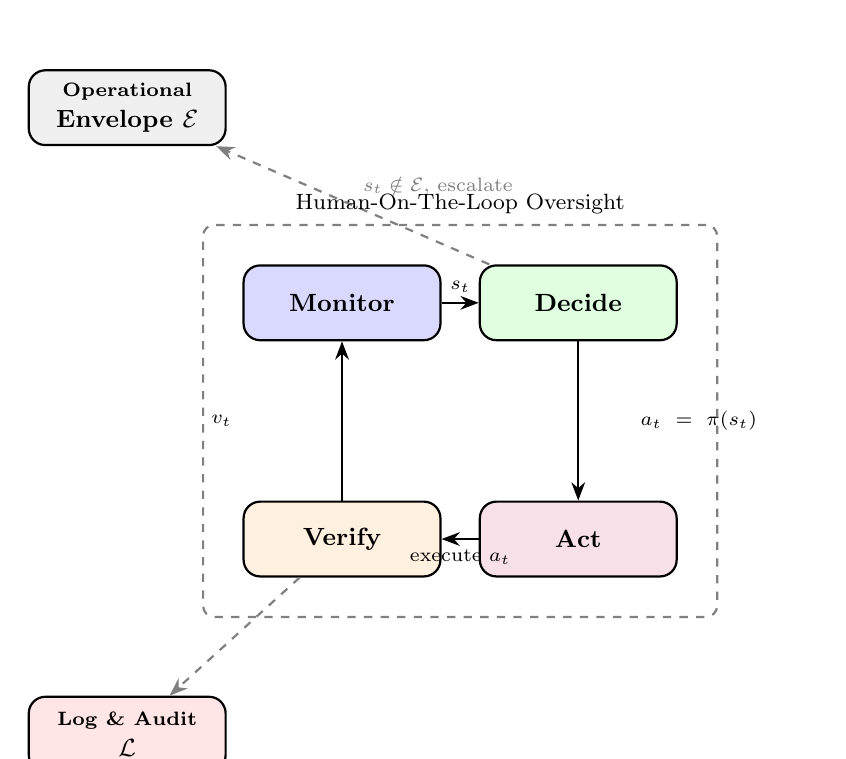
\begin{tikzpicture}[node distance=3cm, >=Stealth, thick,
  phase/.style={rectangle, rounded corners=6pt, draw, fill=blue!10,
    minimum width=2.5cm, minimum height=0.95cm, align=center, font=\small\bfseries},
  annot/.style={font=\scriptsize, align=center, text width=2.8cm}]
  \node[phase, fill=blue!15]   (monitor)  {Monitor};
  \node[phase, fill=green!12,  right of=monitor]  (decide)   {Decide};
  \node[phase, fill=purple!12, below of=decide]   (act)      {Act};
  \node[phase, fill=orange!12, left of=act]        (verify)   {Verify};
  \node[phase, fill=gray!12,   above left=1.5cm and 0.2cm of monitor] (envelope) {\scriptsize Operational\\Envelope $\mathcal{E}$};
  \node[phase, fill=red!10,    below left=1.5cm and 0.2cm of verify]  (log)      {\scriptsize Log \& Audit\\$\mathcal{L}$};

  \draw[->] (monitor) -- node[above, annot] {$s_t$} (decide);
  \draw[->] (decide)  -- node[right, annot] {$a_t = \pi(s_t)$} (act);
  \draw[->] (act)     -- node[below, annot] {execute $a_t$} (verify);
  \draw[->] (verify)  -- node[left,  annot] {$v_t$} (monitor);
  \draw[->, dashed, gray] (decide) -- node[above right, font=\scriptsize] {$s_t \notin \mathcal{E}$, escalate} (envelope);
  \draw[->, dashed, gray] (verify) -- (log);

  \node[draw=gray, dashed, rounded corners, inner sep=0.5cm,
    fit=(monitor)(decide)(act)(verify),
    label={[font=\footnotesize]above:Human-On-The-Loop Oversight}] {};
\end{tikzpicture}
\caption{The Autonomy Loop: five-phase closed-loop cycle. Humans define policy $\pi$, envelope $\mathcal{E}$, and fallback $\mathcal{B}$ at design time; individual loop iterations require no human participation. Dashed edges show the out-of-envelope escalation path and audit logging.}
\label{fig:autonomy-loop}
\end{figure}

\subsection{Key Autonomy Loop Parameters}

\begin{table}[ht]
\centering
\caption{Key operational parameters of the Autonomy Loop.}
\label{tab:parameters}
\begin{tabular}{ll}
\toprule
\textbf{Parameter} & \textbf{Description} \\
\midrule
Operational Envelope $\mathcal{E}$ & Formal bounds within which the system may act autonomously \\
Decision Policy $\pi$ & Algorithm (rule, ML model, PID controller) mapping state to action \\
Authority Level & Maximum magnitude of action the system may take without human approval \\
Monitoring Frequency & How often state $s_t$ is observed; determines reaction latency \\
Escalation Thresholds & Conditions that trigger transition to fallback behaviour $\mathcal{B}$ \\
Fallback Behaviour $\mathcal{B}$ & Response to out-of-envelope states (safe-fail, hold, escalate to human) \\
Action Limits & Hard constraints on action magnitude (e.g., max trade size, max scale step) \\
Audit Trail Depth & Volume of history retained in $\mathcal{L}$ for compliance and forensics \\
\bottomrule
\end{tabular}
\end{table}

%% ================================================================
%% SECTION 5: THE 8-LAYER AUTONOMOUS AI STACK
%% ================================================================
\section{The 8-Layer Autonomous AI Technology Stack}\label{sec:stack}

We decompose the Autonomous AI architecture into eight functional layers, each representing a distinct concern in system design. Unlike the agentic stack (which is organised around reasoning and tool use), the autonomous stack is organised around the closed-loop control cycle and the governance structures that make unsupervised operation safe.

\begin{figure}[ht]
\centering
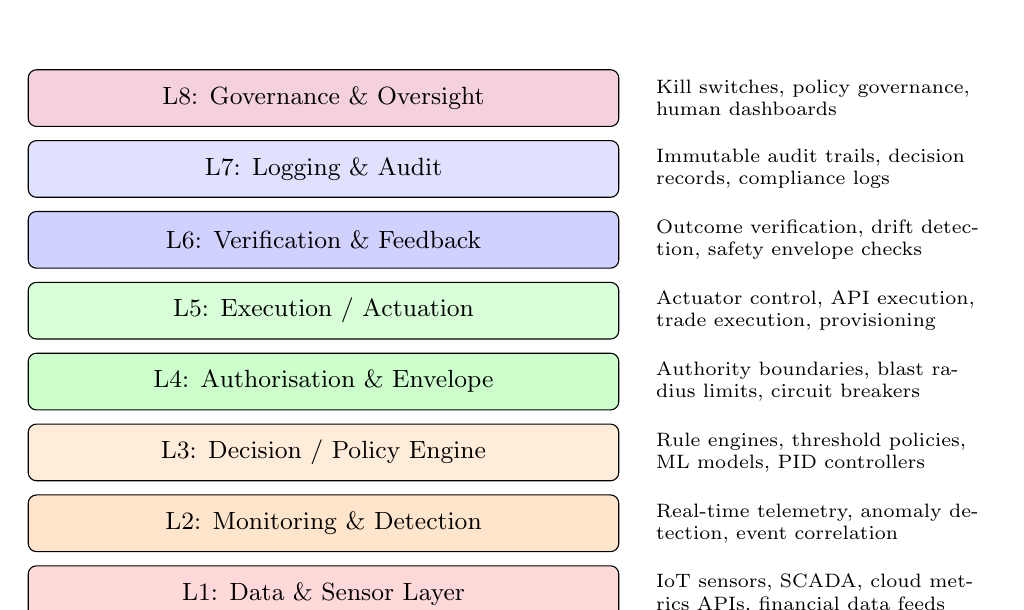
\begin{tikzpicture}[layer/.style={rectangle, draw, rounded corners=3pt,
  minimum width=7.5cm, minimum height=0.72cm, font=\small, align=center},
  label/.style={font=\scriptsize, text width=4.2cm, align=left}]
  \node[layer, fill=purple!18] (l8) at (0, 0)   {L8: Governance \& Oversight};
  \node[layer, fill=blue!12]   (l7) at (0,-0.9)  {L7: Logging \& Audit};
  \node[layer, fill=blue!18]   (l6) at (0,-1.8)  {L6: Verification \& Feedback};
  \node[layer, fill=green!15]  (l5) at (0,-2.7)  {L5: Execution / Actuation};
  \node[layer, fill=green!20]  (l4) at (0,-3.6)  {L4: Authorisation \& Envelope};
  \node[layer, fill=orange!15] (l3) at (0,-4.5)  {L3: Decision / Policy Engine};
  \node[layer, fill=orange!20] (l2) at (0,-5.4)  {L2: Monitoring \& Detection};
  \node[layer, fill=red!15]    (l1) at (0,-6.3)  {L1: Data \& Sensor Layer};

  \node[label, right] at (4.1, 0)   {Kill switches, policy governance, human dashboards};
  \node[label, right] at (4.1,-0.9)  {Immutable audit trails, decision records, compliance logs};
  \node[label, right] at (4.1,-1.8)  {Outcome verification, drift detection, safety envelope checks};
  \node[label, right] at (4.1,-2.7)  {Actuator control, API execution, trade execution, provisioning};
  \node[label, right] at (4.1,-3.6)  {Authority boundaries, blast radius limits, circuit breakers};
  \node[label, right] at (4.1,-4.5)  {Rule engines, threshold policies, ML models, PID controllers};
  \node[label, right] at (4.1,-5.4)  {Real-time telemetry, anomaly detection, event correlation};
  \node[label, right] at (4.1,-6.3)  {IoT sensors, SCADA, cloud metrics APIs, financial data feeds};
\end{tikzpicture}
\caption{The 8-layer Autonomous AI technology stack. Data flows upward (sensor to decision to actuation); governance flows downward (policy to envelope enforcement to logging).}
\label{fig:stack}
\end{figure}

\begin{table*}[ht]
\centering
\caption{The 8-Layer Autonomous AI Stack with representative technologies.}
\label{tab:stack}
\begin{tabular}{cllp{7cm}}
\toprule
\textbf{Layer} & \textbf{Name} & \textbf{Function} & \textbf{Representative Technologies} \\
\midrule
L1 & Data \& Sensor Layer         & Real-world observation            & IoT sensors, SCADA, Prometheus, Kafka, Bloomberg Terminal \\
L2 & Monitoring \& Detection      & State assessment and alerting     & Datadog, Dynatrace, New Relic, Grafana, PagerDuty \\
L3 & Decision / Policy Engine     & State-to-action mapping           & Rule engines, PID controllers, XGBoost, OPA (Open Policy Agent) \\
L4 & Authorisation \& Envelope    & Authority boundary enforcement    & Kubernetes RBAC, rate limiters, circuit breakers (Resilience4j) \\
L5 & Execution / Actuation        & Autonomous action execution       & Kubernetes HPA/VPA/CA, AWS Auto Scaling, Ansible, trading APIs \\
L6 & Verification \& Feedback     & Outcome checking and loop closure & Health checks, canary monitoring, SLO/SLA tracking \\
L7 & Logging \& Audit             & Immutable decision records        & OpenTelemetry, Elasticsearch, Splunk, immutable S3 logging \\
L8 & Governance \& Oversight      & Human-on-the-loop control         & Review dashboards, kill switches, policy management, SOAR \\
\bottomrule
\end{tabular}
\end{table*}

\subsection{Layer-by-Layer Analysis}

\paragraph{L1: Data \& Sensor Layer.}
Every autonomous system begins with observation. In industrial settings, this layer comprises physical sensors (temperature, pressure, flow, vibration) connected via SCADA systems or Distributed Control Systems (DCS). In cloud computing, it comprises metrics APIs (CPU, memory, request rate, error rate) surfaced by Prometheus or CloudWatch. In financial trading, it comprises market data feeds (NYSE, NASDAQ, CME), order book data, and alternative data streams. The key engineering constraint at this layer is \emph{latency}: high-frequency trading requires sub-microsecond data delivery; aircraft autopilots require sensor fusion at $>$100 Hz; cloud auto-scalers operate on 60-second metric windows.

\paragraph{L2: Monitoring \& Detection.}
Raw sensor data is aggregated and analysed to detect conditions that warrant action. This layer implements threshold monitoring, statistical anomaly detection, and event correlation. Modern AIOps platforms (Datadog, Dynatrace, New Relic) apply ML at this layer to reduce false-positive alert rates, but the action triggered by a detected condition is still governed by the pre-defined policy at L3.

\paragraph{L3: Decision / Policy Engine.}
This is the cognitive core of the autonomous system, but it is emphatically not open-ended reasoning. The policy $\pi$ is fully specified before deployment and determines the action for each state. Policy implementations vary by domain: PID controllers in process automation, rule engines (Drools, OPA) in business automation, pre-trained ML classifiers in fraud detection, and discrete-event state machines in CI/CD pipelines. Critically, the policy cannot generate novel strategies; it can only apply its learned or programmed mapping.

\paragraph{L4: Authorisation \& Envelope.}
The authorisation layer enforces the operational envelope $\mathcal{E}$, ensuring that no action exceeds the authority boundary set by humans. This is implemented via rate limiters (maximum API calls per second), position limits (maximum trade size), blast radius controls (maximum number of pods that can be scaled in a single step), and circuit breakers (Resilience4j, Netflix Hystrix) that halt autonomous activity when downstream services exhibit elevated error rates.

\paragraph{L5: Execution / Actuation.}
Authorised actions are executed at this layer. In cloud computing, Kubernetes HPA adjusts pod replica counts; AWS Auto Scaling terminates and launches EC2 instances. In industrial control, DCS controllers send setpoint commands to actuators (valves, motors, pumps). In algorithmic trading, order management systems (OMS) route orders to exchanges via FIX protocol. The execution layer is designed for determinism and reliability: the same authorised action must produce the same effect every time.

\paragraph{L6: Verification \& Feedback.}
After execution, the system verifies that the action achieved its intended effect. In cloud systems, this involves checking that new instances have passed health checks before routing traffic. In industrial control, it involves confirming that the actuator reached the target setpoint within tolerance. In trading, it involves confirming order fills and updating position records. Verification outputs feed directly back to L2, closing the loop.

\paragraph{L7: Logging \& Audit.}
Every decision ($s_t$, $\pi(s_t)$, $a_t$, $v_t$) is recorded in $\mathcal{L}$ for compliance and forensics. Regulatory requirements (MiFID~II, GDPR, FDA audit trail requirements) mandate that this log be tamper-proof and queryable. Modern implementations use append-only object storage (S3 with Object Lock) or distributed ledgers for financial applications.

\paragraph{L8: Governance \& Oversight.}
The governance layer provides the human-on-the-loop interface: dashboards for monitoring system performance, kill switches for emergency halts, policy management tools for adjusting $\pi$ and $\mathcal{E}$, and periodic review workflows for detecting policy drift or bias accumulation. This layer does not participate in the real-time Autonomy Loop but can modify all lower-layer parameters and halt the system at any time.

%% ================================================================
%% SECTION 6: SUB-TYPES OF AUTONOMOUS AI
%% ================================================================
\section{Sub-Types of Autonomous AI}\label{sec:subtypes}

We identify four operationally distinct sub-types of Autonomous AI, differentiated by triggering mechanism, timing, and decision structure.

\begin{table*}[ht]
\centering
\caption{Four sub-types of Autonomous AI with defining characteristics and examples.}
\label{tab:subtypes}
\begin{tabular}{lp{4cm}p{3.5cm}p{4cm}}
\toprule
\textbf{Sub-Type} & \textbf{Trigger} & \textbf{Timing} & \textbf{Examples} \\
\midrule
\textbf{Continuous Control}
  & Continuous feedback signal (sensor reading vs.\ setpoint)
  & Real-time / millisecond loop
  & Aircraft autopilot, cruise control (ACC), power grid balancing, DCS process control, spacecraft attitude control \\
\addlinespace
\textbf{Event-Driven}
  & Discrete event or threshold crossing
  & On-demand / sub-second to minutes
  & Cloud auto-scaling, automated incident response, circuit breakers, self-healing infrastructure, automated failover \\
\addlinespace
\textbf{Scheduled / Pipeline}
  & Time trigger or upstream completion event
  & Scheduled / hours to days
  & CI/CD pipelines, ETL data pipelines, MLOps retraining pipelines, report generation, backup \& archival \\
\addlinespace
\textbf{Autonomous Decision Systems}
  & Application request or market event
  & Per-decision / microseconds to seconds
  & Algorithmic trading, dynamic pricing, content moderation, automated loan decisioning, automated underwriting \\
\bottomrule
\end{tabular}
\end{table*}

\subsection{Continuous Control Autonomy}
Continuous control represents the oldest form of autonomous AI, implemented in aircraft autopilots since the 1930s and industrialised in DCS and PLC (Programmable Logic Controller) platforms throughout the 1970s to 1990s. Modern implementations maintain strict real-time requirements: aircraft attitude control systems operate at $>$100 Hz; power grid frequency controllers must respond within 500 ms to maintain 50/60 Hz stability.

The defining safety property of continuous control systems is the \emph{stability certificate}: Lyapunov stability analysis~\citep{lyapunov1892} can prove, for many control laws, that the system will remain within the operational envelope $\mathcal{E}$ under specified disturbance conditions. This formal verifiability is a key safety advantage over agentic systems.

\subsection{Event-Driven Autonomy}
Event-driven autonomous systems act when a monitored metric crosses a pre-defined threshold. Kubernetes Horizontal Pod Autoscaler (HPA) is the canonical example: when average CPU utilisation across a deployment exceeds 70\%, HPA adds pod replicas; when utilisation falls below 50\%, replicas are reduced. Cloud providers report that approximately 85\% of production cloud workloads employ auto-scaling~\citep{aws2024autoscaling}, making event-driven autonomy the most widely deployed form of AI-driven automation.

Self-healing infrastructure, where Kubernetes replaces failed pods and re-routes traffic automatically, has been shown to reduce Mean Time to Recovery (MTTR) by up to 80\% compared to manual remediation~\citep{netflix2024chaos}. This improvement is achieved without any reasoning or planning: the system simply detects a pod-health-check failure and triggers the pre-defined replacement policy.

\subsection{Scheduled / Pipeline Autonomy}
CI/CD pipelines, MLOps retraining workflows, and ETL data pipelines represent a form of autonomy where the trigger is temporal or graph-based (downstream completion) rather than metric-based. The GitLab State of DevOps 2024 report~\citep{gitlab2024devops} documents adoption at 78\% of software development teams. These systems are autonomous in the sense that they execute multi-step workflows (build, test, deploy, validate) without human approval at each step. However, they remain firmly non-agentic: the workflow graph is static, defined in declarative pipeline configuration (YAML, HCL, Python DAGs), and cannot be modified at runtime.

\subsection{Autonomous Decision Systems}
Autonomous decision systems represent the highest-stakes category: systems that make consequential decisions (trade, approve, remove, price) in real time without human review. Algorithmic trading constitutes 60 to 75\% of US equity market volume~\citep{tabb2024trading}, with high-frequency trading engines operating at nanosecond latencies beyond human reaction time. Content moderation at Meta~\citep{meta2024transparency} autonomously processes approximately 500 million pieces of content per quarter. Automated loan decisioning has compressed approval times from days to seconds at fintech lenders such as SoFi, Lemonade, and Oscar Health.

These systems carry the highest regulatory exposure. Their decision policies ($\pi$) must be fully documented, tested for bias, and, in the EU, subject to human review rights under GDPR Article 22 and the EU AI Act.

%% ================================================================
%% SECTION 7: PLATFORMS AND TOOLS
%% ================================================================
\section{Platforms, Frameworks \& Tools}\label{sec:platforms}

\begin{table}[ht]
\centering
\caption{Cloud auto-scaling and self-healing platforms.}
\label{tab:platforms-cloud}
\begin{tabular}{lll}
\toprule
\textbf{Platform} & \textbf{Provider} & \textbf{Key Capability} \\
\midrule
AWS Auto Scaling                & Amazon   & EC2, ECS, EKS, DynamoDB; predictive scaling \\
Azure VM Scale Sets             & Microsoft & VM + Azure Autoscale for PaaS services \\
GCP Managed Instance Groups     & Google   & Compute Engine + GKE Autopilot \\
Kubernetes HPA / VPA / CA       & CNCF     & Pod and cluster-level auto-scaling \\
HashiCorp Nomad                 & HashiCorp & Workload scheduling; multi-cloud \\
\bottomrule
\end{tabular}
\end{table}

\begin{table}[ht]
\centering
\caption{MLOps and autonomous pipeline platforms.}
\label{tab:platforms-mlops}
\begin{tabular}{lll}
\toprule
\textbf{Platform} & \textbf{Provider} & \textbf{Key Capability} \\
\midrule
Kubeflow        & Google (OSS)   & End-to-end ML pipelines on Kubernetes \\
MLflow          & Databricks     & Experiment tracking, model registry, deployment \\
Apache Airflow  & Apache (OSS)   & DAG-based workflow orchestration \\
Prefect         & Prefect        & Python-native workflow orchestration \\
Dagster         & Dagster (OSS)  & Asset-based data and ML pipelines \\
Argo Workflows  & CNCF (OSS)     & Kubernetes-native workflow engine \\
\bottomrule
\end{tabular}
\end{table}

\begin{table}[ht]
\centering
\caption{AIOps and IT operations platforms.}
\label{tab:platforms-aiops}
\begin{tabular}{lll}
\toprule
\textbf{Platform} & \textbf{Provider} & \textbf{Key Capability} \\
\midrule
Datadog       & Datadog    & Infrastructure monitoring; ML anomaly detection \\
Dynatrace     & Dynatrace  & AIOps; root cause analysis; auto-remediation \\
New Relic     & New Relic  & Observability; AI-assisted anomaly detection \\
PagerDuty     & PagerDuty  & Incident management; automated remediation workflows \\
Splunk XSOAR  & Splunk     & SOAR; security automation playbooks \\
\bottomrule
\end{tabular}
\end{table}

\begin{table}[ht]
\centering
\caption{Industrial control and SCADA platforms.}
\label{tab:platforms-scada}
\begin{tabular}{lll}
\toprule
\textbf{Platform} & \textbf{Provider} & \textbf{Domain} \\
\midrule
Honeywell Experion PKS   & Honeywell  & Refining, chemicals, oil \& gas \\
ABB Ability Symphony Plus & ABB       & Power generation, water utilities \\
Emerson DeltaV           & Emerson   & Batch control, safety systems \\
Siemens SPPA-T3000       & Siemens   & Power plant control \\
OSIsoft PI (AVEVA)       & AVEVA     & Real-time operational data infrastructure \\
\bottomrule
\end{tabular}
\end{table}

%% ================================================================
%% SECTION 8: INDUSTRY USE CASES
%% ================================================================
\section{Industry Use Cases}\label{sec:usecases}

Table~\ref{tab:usecases} summarises the principal production deployments across six industry sectors.

\begin{table*}[ht]
\centering
\caption{Production Autonomous AI deployments across six industry sectors.}
\label{tab:usecases}
\begin{tabular}{llp{5cm}p{4cm}}
\toprule
\textbf{Sector} & \textbf{Use Case} & \textbf{Description} & \textbf{Key Examples} \\
\midrule
\multirow{4}{*}{\textbf{Finance}}
  & Algorithmic Trading        & Fully autonomous trade execution at microsecond speed & Citadel, Two Sigma, Jane Street \\
  & Dynamic Pricing            & Autonomous price adjustment in real time               & Amazon, airlines, Uber \\
  & Automated Fraud Prevention & Auto-block fraudulent transactions in real time        & Visa, PayPal, Stripe Radar \\
  & Automated Underwriting     & Instant loan and insurance decisioning                 & SoFi, Lemonade, Oscar Health \\
\midrule
\multirow{4}{*}{\textbf{Technology}}
  & Auto-Scaling               & Autonomous compute resource scaling                   & AWS, Azure, GCP \\
  & Self-Healing Infrastructure & Automatic failure detection and remediation          & Kubernetes, Netflix \\
  & CI/CD Pipelines            & Automated build, test, and deploy on commit           & GitHub Actions, GitLab CI \\
  & Automated Security Response & Detect and contain threats automatically             & Palo Alto XSOAR, Splunk \\
\midrule
\multirow{3}{*}{\textbf{Energy}}
  & Grid Balancing             & Autonomous supply-demand balancing with renewables    & National Grid ESO, ERCOT \\
  & Smart Building Management  & Autonomous HVAC and energy optimisation               & Siemens, Schneider Electric \\
  & Wind Farm Optimisation     & Autonomous turbine yaw and pitch control              & Vestas, GE, Siemens Gamesa \\
\midrule
\multirow{3}{*}{\textbf{Aviation}}
  & Aircraft Autopilot         & Autonomous flight management; manages 95\% of flight time & Boeing, Airbus \\
  & Air Traffic Flow           & Autonomous conflict detection and flow management     & EUROCONTROL, FAA ATFM \\
  & Satellite Station-Keeping  & Autonomous collision avoidance and attitude control   & Starlink, OneWeb \\
\midrule
\multirow{3}{*}{\textbf{Manufacturing}}
  & Lights-Out Manufacturing   & Fully automated production; no operators on floor     & FANUC, DMG MORI \\
  & Automated Quality Control  & Autonomous inspection at production speed             & Cognex, Keyence, Landing AI \\
  & Predictive Maintenance Actuation & Auto-schedule maintenance on degradation signal  & Siemens MindSphere \\
\midrule
\multirow{3}{*}{\textbf{Retail}}
  & Automated Replenishment    & Autonomous inventory reordering at threshold          & Amazon, Walmart \\
  & Content Moderation         & Autonomous removal of policy-violating content        & Meta (500M actions/quarter) \\
  & Automated Advertising      & Autonomous bid management and placement               & Google Smart Bidding, Meta Advantage+ \\
\bottomrule
\end{tabular}
\end{table*}

%% ================================================================
%% SECTION 9: BENCHMARKS AND EVALUATION
%% ================================================================
\section{Benchmarks \& Evaluation Metrics}\label{sec:evaluation}

Unlike agentic systems, autonomous systems are evaluated along three orthogonal axes: \emph{autonomy} (how much it does without humans), \emph{reliability} (how often it does it correctly), and \emph{decision quality} (how well its decisions match expert judgement).

\begin{table}[ht]
\centering
\caption{Autonomy evaluation metrics.}
\label{tab:metrics-autonomy}
\begin{tabular}{ll}
\toprule
\textbf{Metric} & \textbf{Definition} \\
\midrule
Human Intervention Rate & Fraction of decisions or events requiring human involvement \\
Autonomous Operating Time & Total time operating without human intervention \\
Escalation Rate & Fraction of events escalated to human operators \\
Automation Coverage & Fraction of the total workflow automated end-to-end \\
Mean Time to Autonomous Resolution (MTAR) & Avg.\ time from event detection to autonomous resolution \\
\bottomrule
\end{tabular}
\end{table}

\begin{table}[ht]
\centering
\caption{Reliability evaluation metrics with indicative targets.}
\label{tab:metrics-reliability}
\begin{tabular}{lll}
\toprule
\textbf{Metric} & \textbf{Definition} & \textbf{Target} \\
\midrule
Uptime / Availability        & \% of scheduled time system is operational & $\geq99.9\%$ \\
MTBF                         & Mean Time Between Failures                & Application-specific \\
MTTR                         & Mean Time to Recovery (autonomous)        & $<5$ min (cloud); $<100$ ms (control) \\
False Positive Rate          & Fraction of unnecessarily triggered actions & $<1\%$ (critical systems) \\
False Negative Rate          & Fraction of missed events requiring action  & $<0.1\%$ (safety-critical) \\
\bottomrule
\end{tabular}
\end{table}

\begin{table}[ht]
\centering
\caption{Decision quality metrics.}
\label{tab:metrics-quality}
\begin{tabular}{ll}
\toprule
\textbf{Metric} & \textbf{Definition} \\
\midrule
Decision Accuracy    & Fraction of decisions matching expert judgement \\
Regret Rate          & Fraction of decisions later reversed or corrected \\
Compliance Rate      & Fraction of decisions complying with applicable policy and regulation \\
Latency              & Time from event detection to action execution \\
Revenue / Cost Impact & Financial impact of autonomous decisions (P\&L, costs saved) \\
\bottomrule
\end{tabular}
\end{table}

\subsection{Domain-Specific Performance Data}
Representative performance data from production deployments:
\begin{itemize}
    \item \textbf{Cloud auto-scaling:} AWS predictive scaling reduces over-provisioning by 18 to 45\%; Kubernetes HPA achieves 99.9\%+ uptime across major deployments.
    \item \textbf{Self-healing:} Netflix Chaos Engineering demonstrates MTTR reduction of ${\sim}80\%$ vs.\ manual remediation~\citep{netflix2024chaos}.
    \item \textbf{CI/CD:} Deployment frequency increases of 200+ times and lead time reductions of 99\%+ are documented in the DORA State of DevOps report~\citep{dora2024devops}.
    \item \textbf{Aircraft autopilot:} Manages 95\% of flight time with fatal accident rate $< 0.07$ per million departures (IATA 2024).
    \item \textbf{Algorithmic trading:} HFT market-making reduces bid-ask spreads by 15 to 25\% and provides continuous liquidity~\citep{tabb2024trading}.
    \item \textbf{Dynamic pricing:} Amazon reprices millions of products daily; airlines achieve 5 to 15\% revenue uplift vs.\ static pricing.
\end{itemize}

%% ================================================================
%% SECTION 10: MARKET & ADOPTION DATA
%% ================================================================
\section{Market \& Adoption Data}\label{sec:market}

\begin{table}[ht]
\centering
\caption{Autonomous AI adoption metrics (2024).}
\label{tab:market}
\begin{tabular}{lll}
\toprule
\textbf{Market Segment} & \textbf{Metric} & \textbf{Source} \\
\midrule
Algorithmic Trading           & 60 to 75\% of US equity volume          & TABB Group \\
Global AIOps Market           & ${\sim}\$5.2$B; CAGR ${\sim}20\%$    & IDC / Gartner \\
Cloud Auto-Scaling Adoption   & ${\sim}85\%$ of cloud workloads       & AWS / Azure \\
CI/CD Adoption                & ${\sim}78\%$ of software teams        & GitLab Survey \\
Automated Content Moderation  & ${\sim}10$B actions/quarter (Meta)    & Meta Transparency \\
Dynamic Pricing Adoption      & ${\sim}45\%$ of large retailers       & McKinsey \\
\bottomrule
\end{tabular}
\end{table}

\subsection{Growth Trajectories}
The AIOps market (self-managing IT infrastructure) is projected to grow from \$5.2B (2024) to \$18.4B (2030) at a 20\% CAGR, driven by the increasing complexity of cloud-native architectures and the operational cost of manual incident management. Autonomous trading infrastructure investment continues to grow as regulatory requirements for electronic trading risk controls create barriers to entry that favour established algorithmic participants. Autonomous vehicle technology, while experiencing slower commercial progression than initial projections, has seen Waymo surpass 20 million fully driverless miles, establishing the operational viability of the model.

Key adoption trends:
\begin{itemize}
    \item \textbf{Growing autonomous scope:} Systems are granted increasing authority as operating track records build, resulting in more decisions, higher-value decisions, and broader operational envelopes.
    \item \textbf{AIOps mainstream adoption:} Self-healing, self-scaling infrastructure is now the default configuration for production cloud workloads.
    \item \textbf{Edge autonomy:} Autonomous decision-making is moving to the network edge, enabling sub-millisecond response times in IoT and industrial applications.
    \item \textbf{Regulatory pressure on autonomous decisions:} EU AI Act and GDPR Article 22 are driving investment in explainability and human review mechanisms for automated decision systems.
    \item \textbf{Autonomous-to-agentic transition:} A growing class of systems is augmenting pre-defined autonomous pipelines with LLM reasoning for exception handling, creating hybrid architectures that partially satisfy our formal criterion set.
\end{itemize}

%% ================================================================
%% SECTION 11: RISKS, LIMITATIONS & FAILURE MODES
%% ================================================================
\section{Risks, Limitations \& Failure Modes}\label{sec:risks}

\subsection{Fundamental Limitations}
The architectural properties that make autonomous systems safe, namely bounded scope, pre-defined policy, and formal verifiability, are also their fundamental limitations:

\begin{table}[ht]
\centering
\caption{Fundamental limitations of Autonomous (Non-Agentic) AI.}
\label{tab:limitations}
\begin{tabular}{p{3.5cm}p{9.5cm}}
\toprule
\textbf{Limitation} & \textbf{Description} \\
\midrule
Fixed Scope & Cannot handle situations outside the defined operational envelope $\mathcal{E}$; out-of-envelope events trigger escalation or safe-fail \\
No Novel Reasoning & Cannot reason about new problem types; the policy $\pi$ covers only the situation space anticipated at design time \\
Policy Rigidity & Follows pre-defined $\pi$; may not respond optimally to unprecedented edge cases or distribution shifts \\
Cascading Failures & Autonomous actions can cascade across interconnected systems, amplifying errors at machine speed \\
Lack of Judgement & Cannot exercise contextual judgement in ethically complex or multi-stakeholder situations \\
Opacity of ML Decisions & When $\pi$ is an ML model, individual decisions may not be explainable or auditable at the feature level \\
Over-Reliance Risk & Operators may lose the skills required to perform manual operations when the system fails \\
\bottomrule
\end{tabular}
\end{table}

\subsection{Safety \& Operational Risk Taxonomy}

\begin{table}[ht]
\centering
\caption{Safety and operational risk taxonomy for autonomous systems.}
\label{tab:risks}
\begin{tabular}{p{3cm}p{5cm}p{4.5cm}}
\toprule
\textbf{Risk} & \textbf{Description} & \textbf{Mitigation} \\
\midrule
Flash Crash & Cascading autonomous trading amplifies market moves at extreme speed & Circuit breakers, kill switches, position limits \\
Automation Bias & Operators trust the system excessively and fail to detect or override errors & Regular human review; clear authority boundaries \\
Cascading Automation & One autonomous action triggers others, creating unexpected chains & System decoupling; rate limiting; blast radius controls \\
Silent Failure & System operates within $\mathcal{E}$ but makes subtly incorrect decisions & Outcome monitoring; statistical drift detection \\
Cybersecurity Compromise & Compromise enables autonomous execution of malicious actions & Defence-in-depth; anomaly detection; secure-by-design \\
Bias Amplification & Autonomous decision systems encode and amplify historical biases at scale & Fairness constraints; bias monitoring; regulatory compliance \\
\bottomrule
\end{tabular}
\end{table}

\subsection{The Autonomy-to-Agency Upgrade Risk}
A particularly important risk scenario arises when an autonomous system is upgraded with agentic capabilities, typically by integrating an LLM for exception handling or natural-language goal specification. Such upgrades may inadvertently satisfy one or more of the formal agentic criteria (dynamic tool selection, open-ended reasoning) without the corresponding safety analysis. We propose the following principle:

\begin{proposition}[Upgrade Risk Principle]
Any upgrade of an Autonomous (Non-Agentic) system that causes it to satisfy one or more agentic criteria must be treated as a new system introduction for safety, compliance, and regulatory purposes. The safety certificate of the original autonomous system does not extend to the upgraded system.
\end{proposition}

%% ================================================================
%% SECTION 12: REGULATION & GOVERNANCE
%% ================================================================
\section{Regulation \& Governance}\label{sec:governance}

\begin{table}[ht]
\centering
\caption{Regulatory framework mapping for Autonomous AI systems.}
\label{tab:regulation}
\begin{tabular}{p{4cm}p{8cm}}
\toprule
\textbf{Framework} & \textbf{Relevance to Autonomous AI} \\
\midrule
EU AI Act (2024)~\citep{eu2024aiact}
  & Autonomous decision systems in high-risk domains (finance, employment, credit, education, law enforcement) require conformity assessment, technical documentation, and post-market monitoring. Human oversight mechanisms are mandatory for high-risk AI. \\
GDPR Article 22~\citep{eu2016gdpr}
  & Right not to be subject to purely automated decision-making with legal or similarly significant effects. Requires human review mechanism for automated credit, employment, and insurance decisions. \\
MiFID II / Regulation AT~\citep{mifid2014}
  & Algorithmic trading systems must implement pre-trade risk controls, kill switches, and circuit breakers. Firms must maintain records of all algorithmic orders for five years. \\
SEC Rule 15c3-5~\citep{sec2010}
  & US broker-dealers using algorithmic trading must implement market access risk controls, including order limit checks and erroneous order prevention. \\
ECOA / Fair Lending Laws~\citep{cfpb2023ecoa}
  & Automated credit decisioning must comply with anti-discrimination requirements; adverse action notices must explain the basis for automated rejections. \\
FDA SaMD Guidance~\citep{fda2019samd}
  & Autonomous medical diagnostic and treatment decision support software must be classified as a medical device; higher-risk autonomous clinical decisions require 510(k) clearance or PMA approval. \\
EASA / FAA Regulations
  & Autopilot systems require certification under aviation safety standards (DO-178C for software, DO-254 for hardware); operational approval tied to safety case documentation. \\
\bottomrule
\end{tabular}
\end{table}

\subsection{Governance Best Practices}
Based on the regulatory landscape and production deployment experience, we identify eight governance best practices for autonomous AI systems:

\begin{enumerate}
    \item \textbf{Human-in-the-Loop Escalation:} Define explicit criteria for when the system must pause and request human authorisation; implement and test the escalation path.
    \item \textbf{Kill Switch:} Mandatory ability to immediately halt all autonomous activity; must be accessible to on-call operators and testable without production impact.
    \item \textbf{Authority Boundaries:} Formally document the operational envelope $\mathcal{E}$, authority level, and action limits; review and update as the system's scope evolves.
    \item \textbf{Decision Logging:} Maintain an immutable audit trail $\mathcal{L}$ recording input state, policy applied, action taken, and outcome; retain for the regulatory minimum period.
    \item \textbf{Periodic Review:} Scheduled human review of autonomous decisions to detect policy drift, distributional shift, and bias accumulation.
    \item \textbf{Blast Radius Limitation:} Enforce hard limits on the maximum impact of any single autonomous decision or action cascade.
    \item \textbf{Shadow Mode Testing:} Operate new or modified autonomous systems in parallel with existing processes before granting live authority; compare decisions to human baseline.
    \item \textbf{Rollback Capability:} Where technically feasible, implement the ability to reverse autonomous actions (database transaction rollback, infrastructure state rollback, trade reversal).
\end{enumerate}

%% ================================================================
%% SECTION 13: OPEN PROBLEMS
%% ================================================================
\section{Open Problems \& Future Directions}\label{sec:future}

\subsection{Formal Verification at Scale}
Current formal verification methods (model checking, Lyapunov analysis, runtime verification) scale to relatively simple state spaces. As autonomous systems integrate ML components with high-dimensional feature spaces, formal safety guarantees become computationally intractable. Research in probabilistic verification~\citep{kwiatkowska2020probabilistic} and abstract interpretation offers partial solutions but has not achieved production deployment for safety-critical ML-driven autonomous systems.

\subsection{Distribution Shift and Policy Robustness}
Autonomous policies are validated against the distribution of states observed during testing. When deployed systems encounter out-of-distribution states (market microstructure changes, novel attack patterns, unexpected sensor correlations), policy behaviour is undefined. Detecting distribution shift before it causes unsafe autonomous actions remains an open research problem.

\subsection{The Hybrid Autonomous-Agentic Architecture}
A growing class of production systems integrates autonomous pipelines with LLM-based exception handling. These hybrid systems satisfy the autonomous formal criteria for routine operation but invoke agentic reasoning for out-of-envelope conditions. Developing a formal safety framework for such hybrid architectures, and defining the precise boundary of the agentic component's authority, is a critical open problem.

\subsection{Regulatory Harmonisation}
The EU AI Act, GDPR, MiFID~II, and FDA SaMD represent sector-specific regulatory instruments that were developed before the current generation of autonomous AI. Harmonising these frameworks, and developing sector-agnostic standards for operational envelopes, audit trails, and human oversight mechanisms, would reduce compliance uncertainty and enable broader deployment of safe autonomous AI.

\subsection{Autonomous AI in Multi-Domain Operations}
Modern autonomous systems increasingly span multiple domains: a cloud-native financial trading platform simultaneously operates autonomous infrastructure scaling (technology domain) and autonomous trading (finance domain). The interaction between domain-specific regulatory frameworks and safety requirements for cross-domain autonomous systems has received little systematic study.

%% ================================================================
%% SECTION 14: CONCLUSION
%% ================================================================
\section{Conclusion}\label{sec:conclusion}

This paper has established a formal, criterion-based distinction between Autonomous (Non-Agentic) AI and Agentic AI, two paradigms that are routinely conflated in academic and industry discourse. The six-dimension formal criterion set (goal origin, tool selection, reasoning mechanism, self-correction capacity, memory architecture, and operational scope) provides a practical classification tool with direct implications for safety analysis, regulatory compliance, and system design.

The \textsc{Autonomy Loop} formalises the closed-loop operational cycle of autonomous systems as a five-phase process (Monitor, Decide, Act, Verify, and Loop) in which humans define the policy $\pi$, operational envelope $\mathcal{E}$, and fallback behaviour $\mathcal{B}$ at design time but do not participate in individual loop iterations. This architectural property, policy pre-specification within a bounded envelope, is both the primary safety guarantee of autonomous systems and their fundamental limitation.

Our survey of production deployments documents the extraordinary scale of autonomous AI in operation today: 60 to 75\% of US equity trading volume, 85\% of cloud workloads, 95\% of civil aviation flight time, and 10 billion content moderation decisions per quarter. These systems achieve their operational goals with high reliability precisely because they do not reason openly; they execute pre-verified policies within formally bounded scopes.

The formal distinction introduced here has practical consequences for three communities. For \emph{system designers}, it clarifies when a system design requires the safety analysis procedures of a formal autonomous system versus the guardrail design of an agentic system. For \emph{regulators}, it provides vocabulary to distinguish systems amenable to conformance testing (autonomous) from systems requiring runtime monitoring and probabilistic compliance assurance (agentic). For \emph{safety engineers}, it identifies the precise architectural changes that constitute an ``autonomous-to-agentic upgrade'' and trigger the need for a new safety case.

As AI systems evolve toward hybrid architectures that combine autonomous pipelines with LLM-based reasoning, the boundary formalised here will become increasingly important and, at the same time, increasingly contested. We offer it as a starting point for the community to develop precise, domain-independent standards for the governance of autonomous AI.

%% ================================================================
%% ACKNOWLEDGEMENTS
%% ================================================================
\section*{Acknowledgements}
This paper is part of the \emph{AI Systems Landscape 2026} project. The interactive knowledge base, data, and all supplementary materials are available at \url{https://hameemm.github.io/ai_systems_landscape_2026/} and \url{https://github.com/HAMEEMM/ai_systems_landscape_2026}. The author thanks the open-source and research communities whose work underlies the survey and empirical data presented here.

%% ================================================================
%% BIBLIOGRAPHY
%% ================================================================
\bibliography{references}

\end{document}
